\overlays{4}{
\begin{slide}{Linux}
{\small
Spendiamo ora qualche parola riguardo a Linux:

\onlySlide*{1}{
{\black
Linux era il progetto \emph{personale} di Linus Torvalds, allora
studente all'università di Helsinki (Finlandia), che stava cercando un
sistema operativo abbastanza economico da usare sul cuo computer di
casa, un 386.

Torvalds inizia così lo sviluppo e poi rilascia pubblicamente il suo
lavoro sotto la licenza GPL. Piano piano qualcuno comincia ad usare
Linux. Lo usa, trova dei problemi, e li segnala, o li risolve e spedisce
a Torvalds il suo contributo.

Con il tempo sempre più persone usano Linux, il kernel cresce.
}
}

\onlySlide*{2}{
{\black
Linux e GNU non erano in origine progetti correlati.

Intorno al 1991, GNU era quasi completato ma gli mancava un kernel, e
partì lo sviluppo di Hurd, un microkernel che al giorno d'oggi non è
ancora completamente sviluppato.

Intanto, Torvalds continua a sviluppare il suo kernel.

Qualcuno non collegato nè a Torvalds, nè a GNU, prova a vedere cosa si
ottiene mescolando GNU, a cui manca un kernel, a Linux, a cui manca
tutto il resto.
}
}

\fromSlide*{3}{
{\black
Nasce GNU/Linux... Ed il resto ormai è storia! \emph{;-)}
}
}

\fromSlide*{4}{
\flushright{
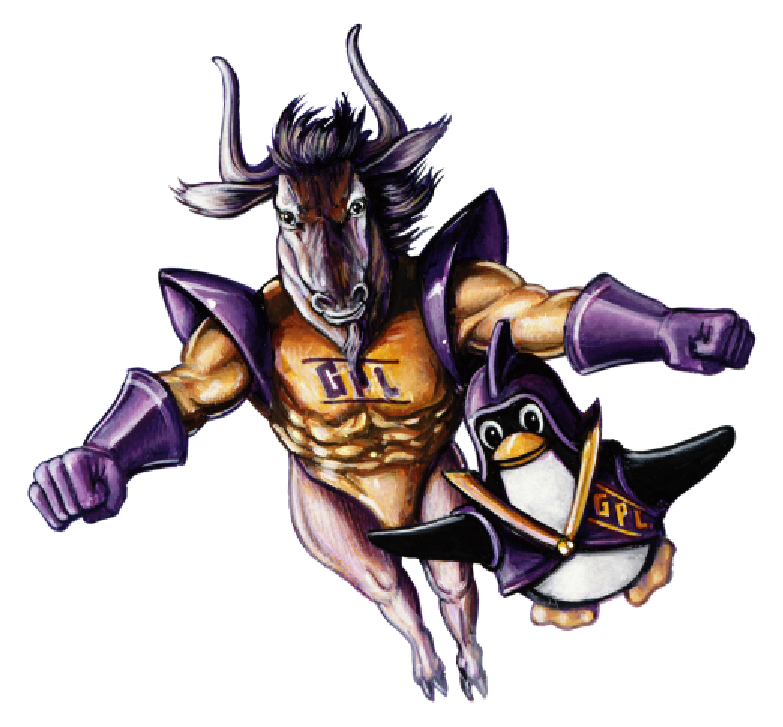
\includegraphics[width=6cm,height=6cm]{immagini/dynamicduo.eps}
}
}

}
\end{slide} }
